% !TEX encoding = UTF-8 Unicode
%!TEX root = thesis.tex
% !TEX spellcheck = en-US
%%=========================================
\chapter{Implementation and Simulation of Sensors}
Using nautical charts, information about other simulated agents and 3D models of installations in sea it is possible to generate realistic sensor data for HIL simulations. This section contains an overview of the implementation of important sensors used on Odin and a brief discussion about how sensor data can be simulated. The Inertial Measurement Unit (IMU) is documented in (\textbf{Evens rapport, trenger referanse?}).

\section{Sensors for Environmental Analysis Implemented on Odin}
\label{SensorOverview}
In section \ref{SensorOverview} a brief overview of the sensors on Odin used for situational awareness above the surface are presented. The overall layout of sensors and system architecture are visualized in Figure \ref{fig:systemArchitecture}.

\begin{figure}[H]
	\begin{center}
		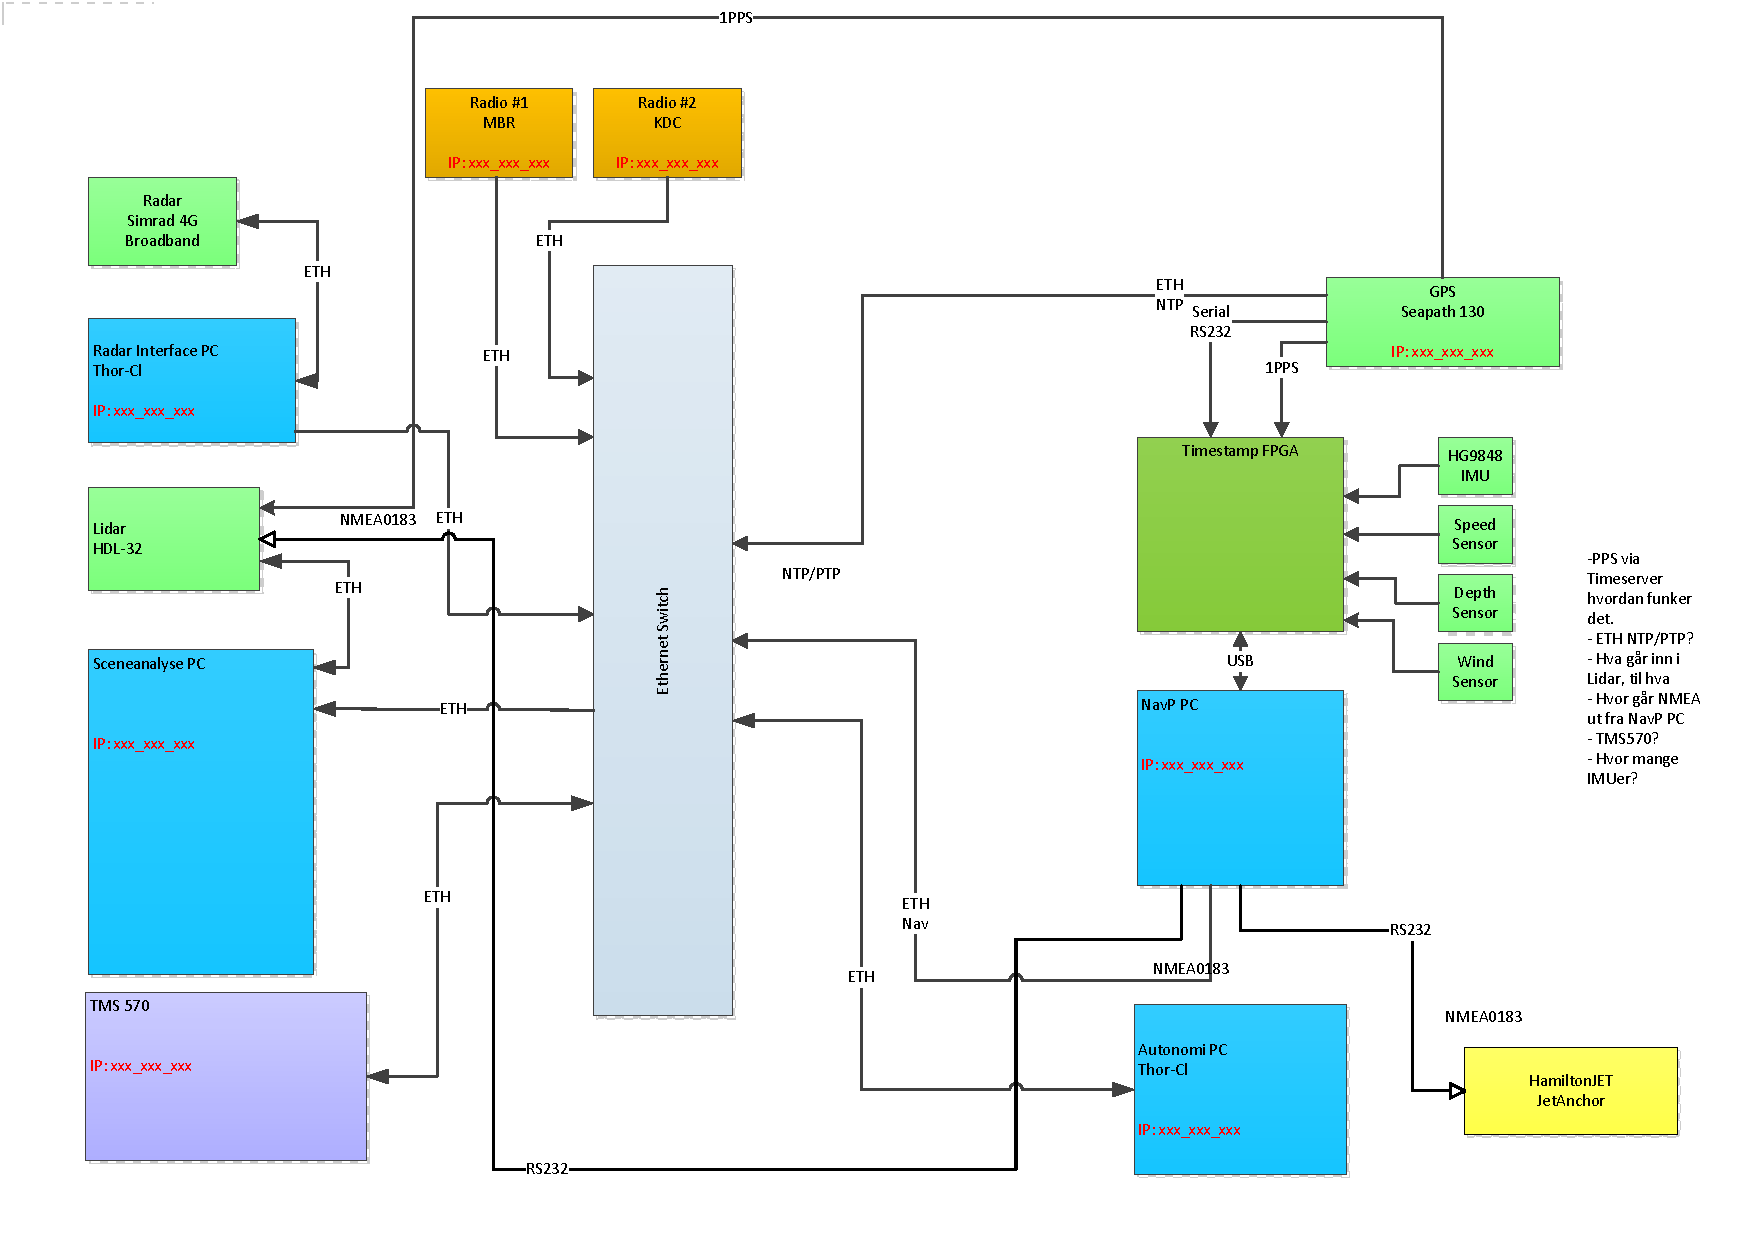
\includegraphics[width = 1\linewidth]{fig/SystemarkitekturOdin.pdf}
		\caption{\textit{Visualization of system architecture and network layout on Odin, including sensors and processing units.} \textbf{A better figure should be made when the final layout is determined!}}
		\label{fig:systemArchitecture}
	\end{center}
\end{figure}

\subsection{Seapath 134 GPS}
The GPS used on Odin is the Seapath 134 developed by Kongsberg Seatex. Combining GNSS signals and IMU data the Seapath 134 gives highly accurate heading, position, heave, roll and pitch measurements (\cite{SeapathManual}). Data is transmitted via standard NMEA protocol over a serial RS232 cable for interpretation by the control system.

\begin{figure}[H]
	\begin{center}
		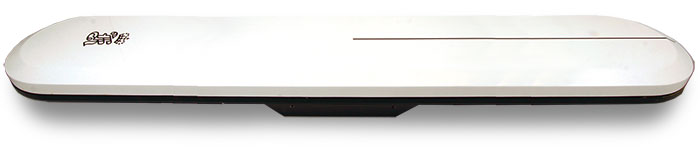
\includegraphics[width = 0.7\linewidth]{fig/Seapath130.jpg}
		\caption{\textit{The Seapath 134 developed by Kongsberg Seatex is used on Odin for position, heading and attitude measurements.}}
		\label{fig:seapath130}
	\end{center}
\end{figure}

\subsection{Radar}
No long text about how radars work is necessary.\\
Introduction to ARPA\\
Thoughts to consider:
\begin{itemize}
	\item Blind zone (minimum detection range).
	\item Range dependent on weather and the shape and orientation of target.
	\item During precipitation clutter a target may or may not be detected. Use randomize function to determine detection? In that case, reproducibility of simulation might be difficult.
	\item Accuracy and how to model errors resulting from inaccuracy.
	\subitem \cite{ARPAmanual} gives great details about possible errors.
	\item Assume (with good reason) that information from ARPA is available as incoming strings following some NMEA like protocol. The information includes at least the detected targets bearing, distance, heading and time. Other possible available data might be time and point of collision, radar cross section (or other target size info), conditions and noise conditions.
\end{itemize}

\newpage
\subsection{Velodyne LiDAR HDL-32E}
\begin{wrapfigure}[14]{l}{0.3\textwidth}
	\vspace{-30pt}
	\begin{center}
		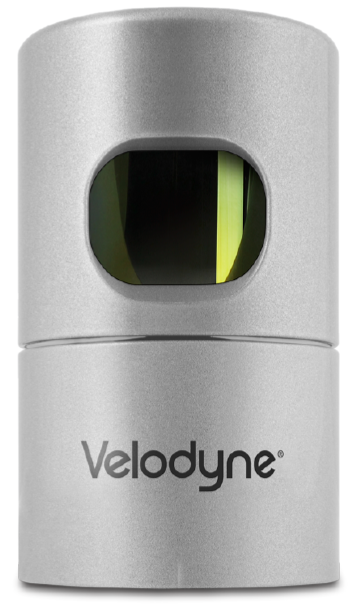
\includegraphics[width= 0.9\linewidth]{fig/VelodyneHDL32Ecase}
		\vspace{-20pt}
		\caption{\it{Velodyne LiDAR HDL-32E used on Odin for above-the-surface 3D analysis.}}
		\label{fig:velodyneCasing}
	\end{center}
	
\end{wrapfigure}
For analysis of the nearby environment above the surface a LiDAR is used to create a 3D point cloud. The model used on Odin is a Velodyne HDL-32E as seen in Figure \ref{fig:velodyneCasing}. A LiDAR can measure the distance to points around the sensor by firing a laser and measure the time it takes for the light to return. The distance is then saved along with the horizontal and vertical angle of the laser, so that the positions of the measured points can be used to generate a 3D model of the nearby environment. Velodyne HDL-32E generates 700,000 points per second with $\pm2$cm accuracy at 80m-100m range. The LiDAR spins around the vertical axis to achieve a $360\degree$ horizontal field of view (FOV), and a combination of 32 lasers stacked vertically yields a $40\degree$ vertical FOV ($+10\degree$ to $-30\degree$). An external GPS should be connected to the LiDAR for time pulse synchronization.

Uncalibrated point cloud data packets are transmitted from the LiDAR over a standard Ethernet cable using UDP. The packet format is well documented in the user manual so that they should be easy to decompose by a custom made point cloud processing unit. A calibration table must be used for vertical correction for each laser. This table is included on a CD delivered with the HDL-32E.
 


\section{Simulation of Sensor Data from Virtual Environment}
The feasibility of simulating realistic sensor data from a virtual environment will be discussed in this section, as well as complexity and benefits regarding simulation of raw versus preprocessed sensor data. Information, hardware and software needed to generate data from each sensor will also be discussed.

\subsection{Simulating Data from GPS}
As the data output of the Seapath 134 follows the well documented NMEA protocol it should be feasible to generate these data based on knowledge of position, speed, heading and attitude. This information should be a result of simulating the boats motion in the virtual environment and is thereby easily accessible.

\subsection{Simulating Data from Radar}
...

\subsection{Simulating Data from LiDAR}
The protocol of the data transfer from Velodyne HDL-32E is well documented. Given a 3D model of the surrounding environment with easy access to angle and distance calculations it should be feasible to generate a realistic point cloud. The point cloud can be represented as data packets using the HDL-32E protocol and sent over Ethernet to the interface between HIL simulator and the control system. This way it would be possible to simulate raw sensor readings from the HDL-32E. This is assumed to be beneficial to the developers of the simulated vehicle as a larger chain of HW/SW can be tested in the simulated environment.	

\textbf{Something about preprocessed data here}.

- \textit{Should the GPS used for clock synchronization also be simulated or could we use the one on the vehicle being tested?}. It is assumed that the system including simulator and hardware is synchronized in time using either NTP or PTP network timing. A real or simulated GPS is therefore not necessary for time synchronization.



\subsection{Raw vs Preprocessed Sensor Data}
Complexity and benefits regarding generating raw data versus preprocessed information.







